\documentclass{article}
\usepackage[utf8]{inputenc}

\title{Lab 4 - Ramsauer-Townsend Effect}
\author{Oisín Peppard}
\date{March 2018}

\usepackage{natbib}
\usepackage{graphicx}
\usepackage[a4paper, total={6in, 8in}]{geometry}
\usepackage{float}



\begin{document}

\maketitle

\begin{center}
    

\section*{Abstract}
This experiment looks at the quantum mechanical Ramsauer-Townsend effect. This theory describes the scattering of low energy electrons by a noble gas, where the theory proposed by Newtonian mechanics fails. A thyratron is used to fire electrons through xenon gas and observe their scattering. The gas is then supercooled with liquid nitrogen. Graphs of the Plate Current, with and without the liquid nitrogen, versus the Voltage were plotted. This illuminated the energy level for minimum scattering. It was found to be $1$V $\pm 0.01$V and 1eV energy. This corresponds to a De Broglie wavelength of 1.23nm. The maximum and minumum values of mean free path were found to be $0.722$m $\pm0.001$m and $0.0434$m $\pm0.001$m respectively. The Contact Potential Difference was investigated and found to be 0.6V $\pm$ 0.03V
\end{center} 


\section*{Theory and Equations}
\subsection*{The Ramsauer-Townsend effect}
In classical mechanics, the probability of a particle being scattered by a central force should be independent of the incident energy. The canonical example given is that a billiard ball is no more or less likely to collide and be scattered by another ball for different velocities and kinetic energies. A different behaviour was observed by Carl Ramsauer and John Sealy Townsend when low energy electrons were passed through a noble gas. It was observed t  hat the scattering cross section was a minimum for an unexpected particular value of kinetic energy. It was not until quantum mechanical theories were developed, and the wave-nature of the electron discovered that this could be explained. Simplifying to the one-dimensional case, an electron is described as a wave packet of discrete energy. Its interaction with a xenon atom is considered to be this wave packet approaching a potential well. It is predicted that the wave will be reflected twice. First at the step down and then again at the step up. If the two reflected waves interfere destructively, no scattering should occur. This implies that for certain electron wavelengths and therefore energy level, the scattering will be a minimum. This coincides with a wavelength being a multiple of the well width. This experiment uses a thyratron to fire electrons through very low pressure xenon. If an electron is scattered it will hit the shield electrode and contribute to the shield current $I_s$. Unscattered electrons pass through to the plate electrode, and become plate current $I_p$. When the xenon gas is frozen out with liquid nitrogen, we meausre a ratio $f$ of the of plate to shield current as a function of accelerating voltage V. 
\[f(V) = \frac{I_p^*(V)}{I_s^*(V)}\]
The * in this equation indicates the current measurements with frozen out xenon. This means we can write 
\[I_p^* = f(V)I_s^*\]
When gaseous xenon is present, as in our first set of measurements, there will be a probability $P_s$ that the electron will be scattered to the shield electrode. We amend the above equation to take this into account.
\[I_p(V) = f(V)I_s(V)(1-P_s)\]
Finally we can express the desired scattering cross section $P_s$ as a function of measurable quantities.
\begin{equation}
    P_s = 1 - \frac{I_pI_s^*}{I_sI_p^*}
\end{equation}
The probability $P$ that an electron is scattered by a medium depends on its mean free path $\lambda$ and the distance $l$ it travels through the xenon i.e. the length of the thyratron chamber. it is given by
\[P = 1-e^{-\frac{l}{\lambda}}\]
Finally, we use this to determine a formula for the current, i.e. number of scattered electrons per second. 
\begin{equation}
    I_{scattering} = PI = (1-e^{-\frac{l}{\lambda}})
\end{equation}

\subsection*{Contact Potential}
In the latter part of this experiment, we attempt to determine the kinetic energy of the electron. This is given as 
\[T = eV_{eff}\] and
\[V_{eff} = V + V_c + \bar{V}\]. $V$ is the effective accelerating voltage varied in the experiment, $V_c$ is the contact potential difference generated by the potential difference across the two metals in contact, and $\bar{V}$ is the energy resultant from thermionic emission of "cathode rays". These values can be found by reversing the polarity and measuring $I_s^*$ and $V$. We can derive a relationship between these quantities.
\[\log{I_s^*} = \log{I_0} - \frac{3V}{2\bar{V}}\]
By plotting $I_s^*$ against $V$ we can determine the contact potential $V_c$ from the point of intersection of the two generated lines, and Thermionic emission energy from the slope of the steeper line

\section*{Apparatus and method}
\begin{figure}[H]
    \centering
    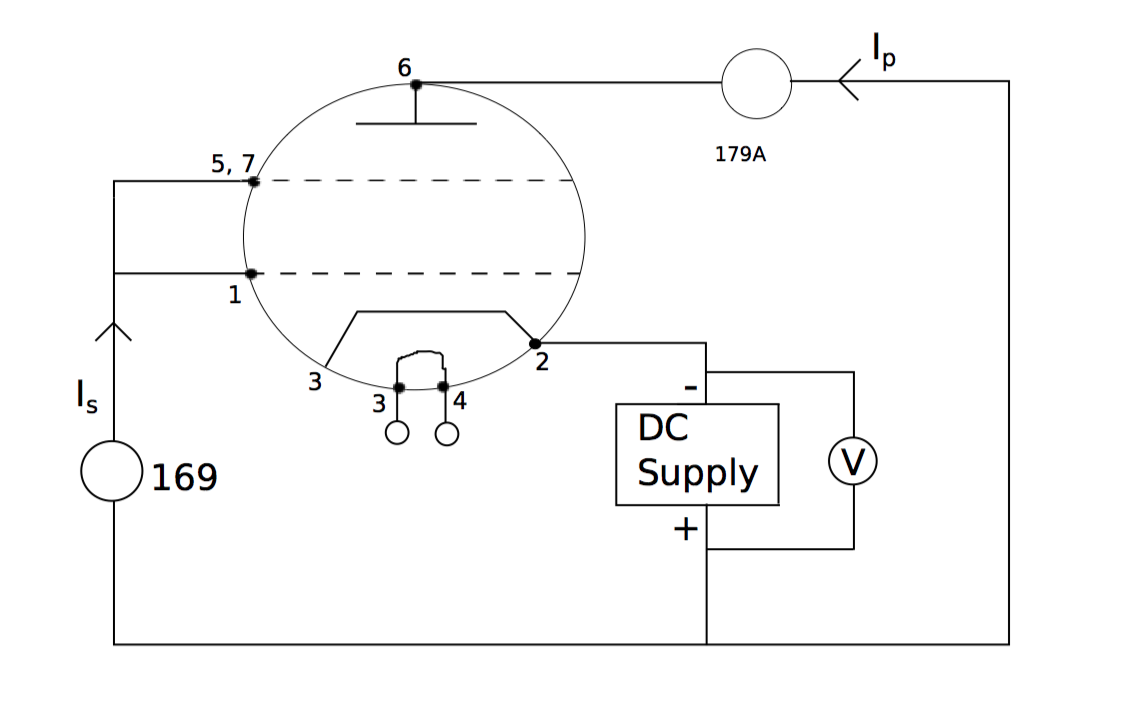
\includegraphics[scale = 0.25]{diagram.png}
    \caption{Diagram of Circuit}
    \label{fig:apparatus}
\end{figure}
The apparatus was set up as shown in Fig (1). The direct current power supply was varied in voltage and the corresponding shield and plate currents measured to obtain $I_s$ and $I_p$. This was then repeated with the thyratron submerged in liquid nitrogen to obtain $I_s^* $and$ I_p^*$. For the final part of the experiment, we reverse the polarity of the accelerating potential so that the electrons are instead decelerated. We once again measure $I_s^*$ while varying Voltage.

\section*{Results}
\begin{figure}[H]
    \centering
    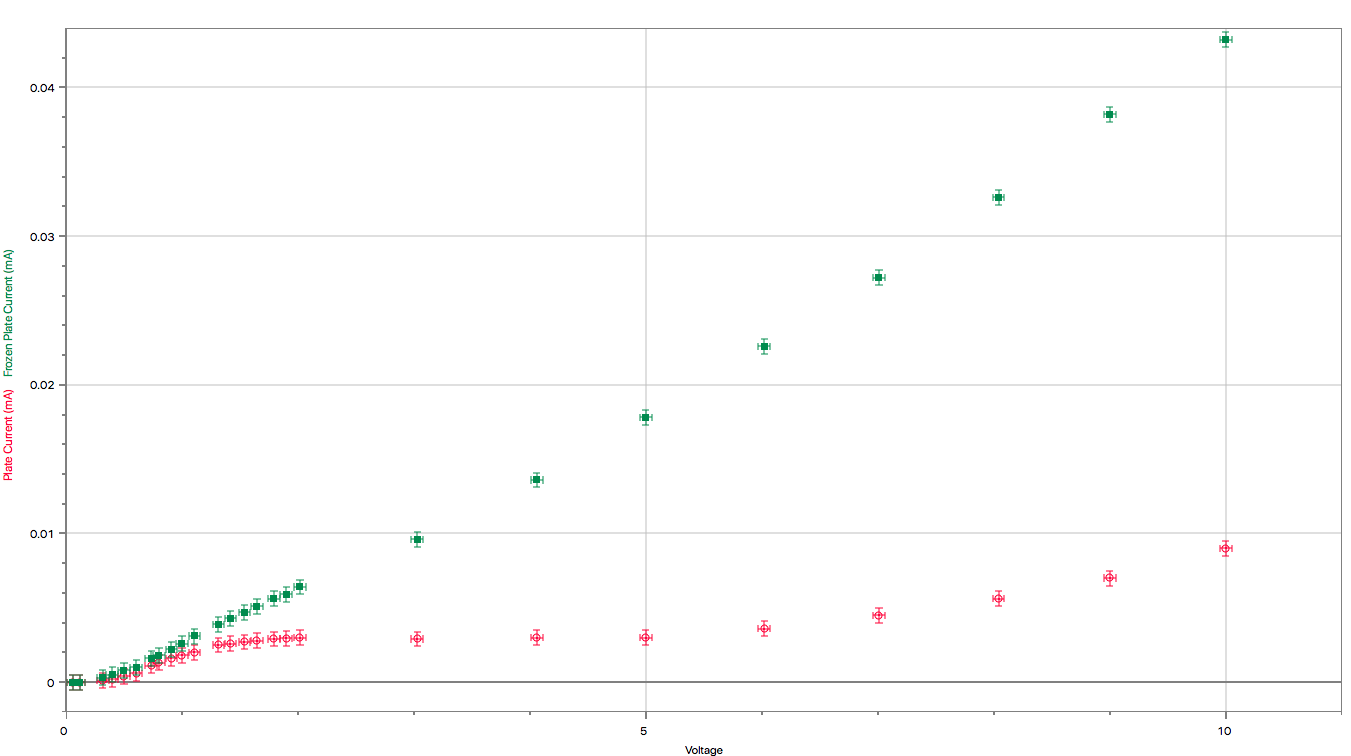
\includegraphics[scale = 0.3]{1.png}
    \caption{Graph of $I_p$ (green) and $I_p^*$ (red) vs. Voltage}
    \label{fig:1}
\end{figure}
\begin{figure}[H]
    \centering
    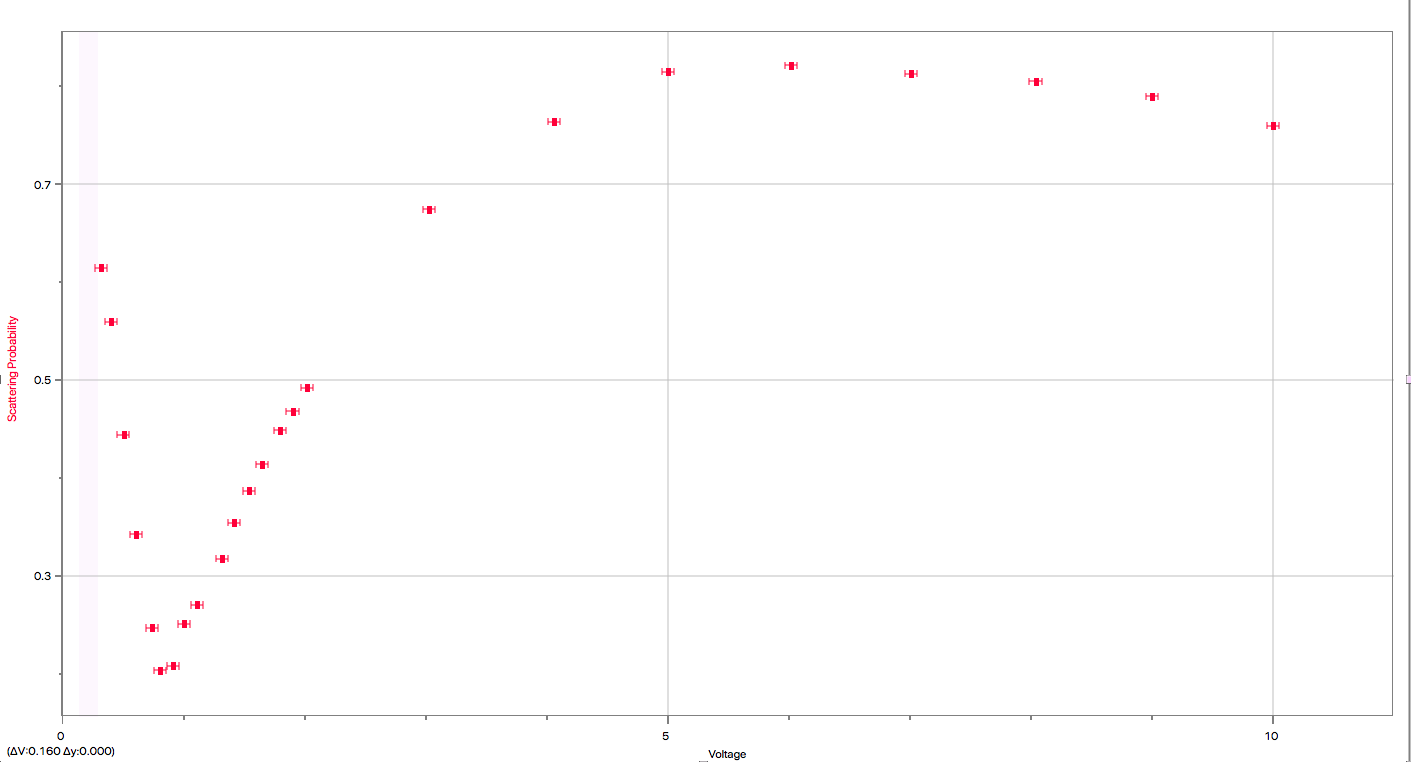
\includegraphics[scale = 0.3]{2.png}
    \caption{Graph of Scattering probability vs. Voltage}
    \label{fig:2}
\end{figure}
\begin{figure}[H]
    \centering
    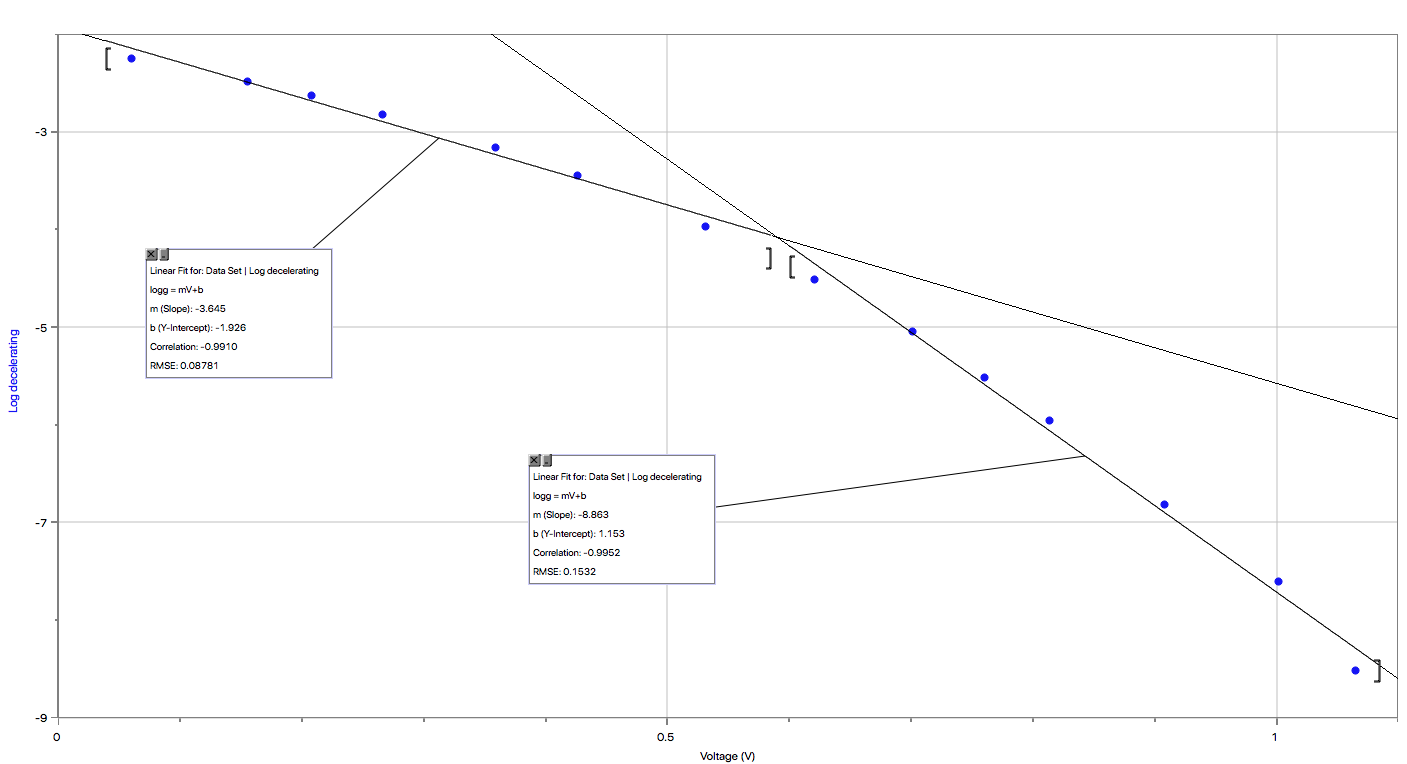
\includegraphics[scale = 0.3]{3.png}
    \caption{Graph of decelerated $I_p^*$ vs. Voltage}
    \label{fig:3}
\end{figure}


\section*{Error Analysis}
The error in both current measurements, $\Delta I$ was taken to be $\pm 0.001$V. The error in input Voltage $\Delta V$ was taken to be $\pm 0.001$V. The subsequent errors in derived logarithmic functions were computed using the standard Gaussian error analysis and the data sets modified to include them in the plots.

\section*{Discussion and conclusions}
It can be clearly seen in Fig (2) that the presence of Xenon significantly effects the scattering cross section of the incident electrons. For low voltage, the graphs of $I_p$ and $I_p^*$ appear to increase similarly, but as Voltage is increased, very few of the electrons reach the plate.

When the scattering probability is graphed against voltage, we see that scattering is a minimum for 1V $\pm$ 0.01V and therefore 1eV energy. By using De Broglie's equation \[\lambda = \frac{h}{p}\] with $p$ meaning momentum and $\lambda$ being wavelength, and considering \[p = \sqrt{2Em_e}\] where $E$ is the energy and $m_e$ the electron's mass, we can calculate the wavelength of the electron for destructive interference to occur within the potential well of the Xenon atom with \[\lambda = \frac{h}{\sqrt{2Em_e}}\] to be 1.23nm.

The maximum and minimum values of mean free path were found to be $0.722$m $\pm0.001$m and $0.0434$m $\pm0.001$m respectively.

The Contact Potential Difference was investigated and found to be 0.6V $\pm$ 0.03V

\end{document}